\documentclass[sigconf]{acmart}

\usepackage{booktabs} % For formal tables
\usepackage[normalem]{ulem}
% Copyright
\setcopyright{none}

\usepackage{ifthen}
\usepackage[normalem]{ulem} % for \sout
\usepackage{xcolor}
\usepackage{amssymb}

\newcommand{\ra}{$\rightarrow$}
\newboolean{showedits}
\setboolean{showedits}{true} % toggle to show or hide edits
\ifthenelse{\boolean{showedits}}
{
	\newcommand{\ugh}[1]{\textcolor{red}{\uwave{#1}}} % please rephrase
	\newcommand{\ins}[1]{\textcolor{blue}{\uline{#1}}} % please insert
	\newcommand{\del}[1]{\textcolor{red}{\sout{#1}}} % please delete
	\newcommand{\chg}[2]{\textcolor{red}{\sout{#1}}{\ra}\textcolor{blue}{\uline{#2}}} % please change
}{
	\newcommand{\ugh}[1]{#1} % please rephrase
	\newcommand{\ins}[1]{#1} % please insert
	\newcommand{\del}[1]{} % please delete
	\newcommand{\chg}[2]{#2}
}

\newboolean{showcomments}
%\setboolean{showcomments}{true}
\setboolean{showcomments}{true}
\newcommand{\id}[1]{$-$Id: scgPaper.tex 32478 2010-04-29 09:11:32Z oscar $-$}
\newcommand{\yellowbox}[1]{\fcolorbox{gray}{yellow}{\bfseries\sffamily\scriptsize#1}}
\newcommand{\triangles}[1]{{\sf\small$\blacktriangleright$\textit{#1}$\blacktriangleleft$}}
\ifthenelse{\boolean{showcomments}}
%{\newcommand{\nb}[2]{{\yellowbox{#1}\triangles{#2}}}
{\newcommand{\nbc}[3]{
 {\colorbox{#3}{\bfseries\sffamily\scriptsize\textcolor{white}{#1}}}
 {\textcolor{#3}{\sf\small$\blacktriangleright$\textit{#2}$\blacktriangleleft$}}}
 \newcommand{\version}{\emph{\scriptsize\id}}}
{\newcommand{\nbc}[3]{}
 \renewcommand{\ugh}[1]{#1} % please rephrase
 \renewcommand{\ins}[1]{#1} % please insert
 \renewcommand{\del}[1]{} % please delete
 \renewcommand{\chg}[2]{#2} % please change
 \newcommand{\version}{}}
\newcommand{\nb}[2]{\nbc{#1}{#2}{orange}}

\definecolor{accolor}{rgb}{0.4,0.6,0.2}
\definecolor{frcolor}{rgb}{0.5,0.7,0.9}
\newcommand\ac[1]{\nbc{AC}{#1}{accolor}}
\newcommand\fr[1]{\nbc{FR}{#1}{frcolor}}
\usepackage{wasysym}
\newcommand\yesml[1]{\nbc{ML {\textcolor{yellow}\sun}}{#1}{mircolor}}

\begin{document}

\title{Iroko: Predictive Datacenter Congestion Control}

\author{Anand Jayarajan}
\affiliation{%
  \institution{University of British Columbia}
}
\email{anandj@cs.ubc.ca}

\author{Michael Przystupa}
\affiliation{%
  \institution{University of British Columbia}
}
\email{michael.przystupa@gmail.com}

\author{Robert Reiss}
\affiliation{%
  \institution{University of British Columbia}
}
\email{rreiss@cs.ubc.ca}

\author{Fabian Ruffy}
\affiliation{%
  \institution{University of British Columbia}
}
\email{fruffy@cs.ubc.ca}

\begin{abstract}
Datacenter networks have become a hotbed of network research in the past 
decade. Many works have been published on improving bisection bandwidth, cost, 
and latency. As a core contribution of this research, centralized scheduling 
has entered the stage as a dominant strategy to manage flows. Benefitting from 
a global view and full control over the network, centralized schedulers are 
able to enforce fine-grained traffic control, frequently achieving near-optimal 
bandwidth optimization. However, modern congestion control algorithms and 
schedulers are still fundamentally reactive. Many algorithms are designed to 
only respond to packet loss or significant increase in latency, not to actively 
prevent it.
In this project, we plan to explore the opportunities of employing a preemptive 
and tightly controlling central network scheduler. By enforcing traffic limits 
and admission control, the scheduler is able to proactively steer the flow of 
traffic. The notion of "knowledge" and predictive analysis in networks is a 
growing trend in research, which we intend to leverage in this system.

We investigate the potential in such a new form of interactive congestion 
control and analyze it against state-of-the-art solutions. Our tool of choice 
to model our system is Mininet, a rapid prototyping emulator for datacenter 
networks. We will compare our "Iroko" system against established TCP-congestion 
systems such as Hedera and DCTCP. Based on the findings, measurement results, 
and effectiveness of our reinforcement learning technique, we will reassess the 
feasibility and prospects of a predictive congestion control algorithm.
\end{abstract}



\keywords{TCP, Congestion Control, SDN, Datacenter}


\maketitle


%%%%%%%%%%%%%%%%%%%%%%%%%%%%%%%%%%%%%%%%%%%%%%%%%%%%%%
\section{Introduction}
\label{sec:intro}
Initially, research in network congestion was dominated by the assumption of a decentralised, autonomous network - end-hosts only have control over the amount of traffic they send, and are unaware of the intentions or traffic rates of their peers. Similarly, switches and routers are unaware of global traffic patterns and only forward based on their local notion of optimality.

In line with these assumptions, TCP was designed to optimize traffic globally on a simple fairness principle: nodes react to packet loss and assume that others will behave accordingly. An equilibrium is reached when all end-hosts achieve a traffic rate that, in sum, conforms to the maximum available bandwidth of the most congested link.
TCP works well  in scenarios where many different distrustful participants compete for limited bandwidth. Still, TCP is a \textit{reactive protocol}; the fact that packet loss and latency increases occur in the network already indicates a problem. Packet loss is primarily due to overflowing queues in forwarding elements, implying that traffic has not been optimally distributed. Ideally, a network should always be "zero-queue", i.e., latency will merely be induced by propagation, and not queuing delay. 

Queueing has generally not been a dominating issue in wide-area and enterprise networks, as traffic is sufficiently distributed and diverse, with only few "hot" target hosts.~\cite{hedera, microte} Traffic optimization is a substantial challenge; network operators have no control over the individual network elements nor its participants. Under these conditions, TCP and its extensions can be considered a best-effort solution.

Developments in the past decade have changed the general networking environment. Datacenters have emerged as an exciting new research frontier, posing novel  design challenges and opportunities.
Driven by minimization of costs and maximization of compute power, data centers must  run at maximum utilization to achieve an optimal compute/cost ratio. Inefficient routing can quickly lead to bufferbloat~\cite{bufferbloat} and the eventual collapse of a high-load network, requiring more sophisticated approaches to solve congestion control. 
On the other hand, operators now have the ability to freely control and adapt their network architecture, leading to highly customized systems and fine-grained optimization. As a result , Software-Defined Networking (SDN) has emerged as a new networking paradigm. Moving away from the principle of distributed communication and routing, SDN introduces the notion of "centralized management". A single controller with global knowledge is able to automatically modify and adapt the forwarding tables of all switches in the network, while notifying end hosts of changes in the network.
These two new trends in system design facilitated impactful new innovation opportunities in the space of TCP congestion research. Traffic can now be managed in a  \textit{centralised} fashion based on \textit{global knowledge} of the entire topology and traffic patterns.
A new line of centralised schedulers has emerged that  can achieve close to optimal bandwidth utilization.~\cite{hedera, fastpass, microte, b4, dionysus}
However, these schedulers are still  \textit{reactive}  in nature. The central controller responds to changes in the network or requests by applications, which may cost valuable roundtrip latency. Often, short-term flows or bursts are unaccounted for, which causes undesirable packet loss and backpropagating congestion. 

A much more desirable solution is a global, centralised arbiter which is able to predict and fairly distribute flows in the network before bursts or congestion occurs. By treating the network’s compute and forwarding power as a single finite resource, a controller acts like the OS scheduler distributing CPU time slices to processes. This design approach follows SDN’s aspiration of introducing operating systems abstractions to the networking domain space.


In this project, we plan to explore the possibilities of a centralised, proactive flow scheduler. We ask ourselves the following research questions:
\begin{enumerate}
\item Is it possible to design a centralised token-based scheduling network?
\item Is it possible to predict traffic and preemptively schedule flows and token distribution in a datacenter context?
\item Using this approach, are we able to achieve better performance and utilization than existing solutions?
\end{enumerate}

In the scope of this course, we attempt to answer question 1 and design a simple token-based scheduler in Mininet. If successful, we will benchmark our results and evaluate the level of utilization compared to contemporary scheduling systems.



%%%%%%%%%%%%%%%%%%%%%%%%%%%%%%%%%%%%%%%%%%%%%%%%%%%%%%%
\section{Motivation}
\label{sec:motivation}
Several recent contributions in networking research 

\paragraph{Software-Defined Networking}
With the advent of Software-Defined Networking (SDN), operators now have the 
ability to freely control and adapt their network architecture, leading to 
highly customized systems and fine-grained optimization.~\cite{sdn_road}

Moving away from the principle of distributed communication and routing, SDN 
introduces the notion of "centralized management". A single controller with 
global knowledge is able to automatically modify and adapt the forwarding 
tables of all switches in the network, while notifying end hosts of changes in 
the network.
This full architectural control and centralized management facilitated new 
opportunities in the space of TCP congestion research. Traffic can now be 
managed in a  \textit{centralized} fashion based on \textit{global knowledge} 
of the entire topology and traffic patterns.

\paragraph{Centralized Scheduling and Congestion Control}
A new line of centralized schedulers has emerged that can achieve close to 
optimal bandwidth utilization.~\cite{hedera, fastpass, microte, b4, dionysus}
However, these schedulers are still  \textit{reactive}  in nature. The central 
controller responds to changes in the network or requests by applications, 
which may cost valuable round-trip latency. Often, short-term flows or bursts 
are unaccounted for, which causes undesirable packet loss and back-propagating 
congestion.

\paragraph{Admission-control systems}
In parallel, admission-control-based approaches have gained traction as a 
viable alternative to the conventional burst-and-backoff mechanism of 
TCP.~\cite{expresspass, fastpass, perc}
The idea of admission control and service guarantees in networks is not 
new.~\cite{access_limit, access_limit2}. However, such designs traditionally 
aim to assure quality and bandwidth guarantees in a contentious, decentralized, 
and untrusted environments such as the internet. In a datacenter, these 
conditions do not apply. End-hosts are generally considered reliable and 
restricted in behaviour, which allows for great simplification of enforcement 
and prioritization policies.

\paragraph{Predictability of traffic}



%%%%%%%%%%%%%%%%%%%%%%%%%%%%%%%%%%%%%%%%%%%%%%%%%%%%%%
\section{Design / Proposed Approach}
\label{sec:design}

\subsection{Overview and Goals}
In our initial simple system, "Iroko", a centralized controller regulates all 
node traffic by rate-limiting end-hosts. We have opted for a centralized 
manager in favor of a distributed protocol to leverage the advantages of a 
global network view.~\footnote{For now, we do not expect our design to scale up 
to thousands of switches. Iroko is intended for small to mid-tier size data 
centers, which may benefit from a simplistic, centralized scheduling model.}
By polling each switch individually for port and utilization statistics we are 
able to infer a global traffic matrix, which we can amalgamate with static 
routing and topology information. 

Iroko guarantees minimal congestion and low average access latency. Reducing 
network-global packet loss and jitter is the priority and objective function of 
the arbiter, which will enforce these goals by restricting host bandwidth. In 
an ideal Iroko system, packet-loss will only rarely, if ever, occur. In respect 
to the free lunch theorem we aim to trade off maximum bandwidth utilization for 
optimal system stability and reliable latency.

It is important to note that routing decisions are not in the current scope of 
Iroko. While it may certainly beneficial to include dynamic and adaptive 
routing decisions in a predictive scheduler, we do not include these features 
in the current system due to time and complexity limitations. Iroko operates on 
static flow routes defined and generated by ECMP. It is assumed that these 
routes will not vary substantially and that the computed ECMP forwarding hash 
is consistent.


\subsection{Controlling traffic flow}
Rate-limiting is performed on the granularity of the IP protocol, allowing us 
to restrict traffic to specific hot regions and to package flows into groups.
End-hosts are guaranteed a limited amount of bandwidth which they may send to 
each destination address. The traffic window size for any flow is calculated 
based on the host's current traffic availability. Total bandwidth of a group of 
flows may never exceed the imposed bandwidth limitation, but nodes are free to 
distribute the allocated resources on singular subflows.

The central arbiter enforces these bandwidth and access limitations by 
assigning "tokens" to nodes. These tokens are plain information packets 
specifying the affected destination address flow, its bandwidth guarantee, and 
the expiration time. Tokens act as the rate-limiter of the system and form a 
queue each end-host will cycle through.

When a node opens a flow, it will look up the current bandwidth restriction for 
the destination IP in its token database and calculate the maximum congestion 
window possible for the particular TCP connection. In our simple design, flows 
are always assigned a fair fraction.

Once a token has expired for a particular flow-group, the restrictions of the 
next token in the queue will be applied. This mechanism is the underlying basis 
for a predictive access control algorithm and does not require any application 
level modification. On end-hosts, only the transport layer services will have 
to be modified.

\subsection{Adapting traffic flow}

Initially, the controller will compute optimal route configuration based on the 
topology and link bandwidth using a simple heuristic bin-packing approach. 
End-hosts will be initialized with a fixed low-to-medium bandwidth guarantee 
that will be adjusted over time. This bandwidth guarantee will be below the 
host's proportional bi-section bandwidth that would be used to reach any other 
host. That is, if every end host transfers using the full bandwidth initially 
allocated to it,  there would be no dropped packets due to congestion.

Of course, this would vastly underutilize network resources, thus the 
controller will dynamically adjust these allocations to ensure that hosts that 
require the bandwidth are allocated it, while host that are not currently 
utilizing all their allocated bandwidth have their allocated bandwidth reduced. 
To avoid starving hosts, some small amount of bandwidth must always be 
allocated to a given host even if it not utilizing network resources. Thus, the 
network, by design, will never reach 100\% utilization.

Conversely however one should rarely see dropped packets due to network 
congestion. Furthermore, the controller must be able to react quickly to 
changing bandwidth needs for hosts. Ideally, using a predictive method.

\begin{figure}
\centering
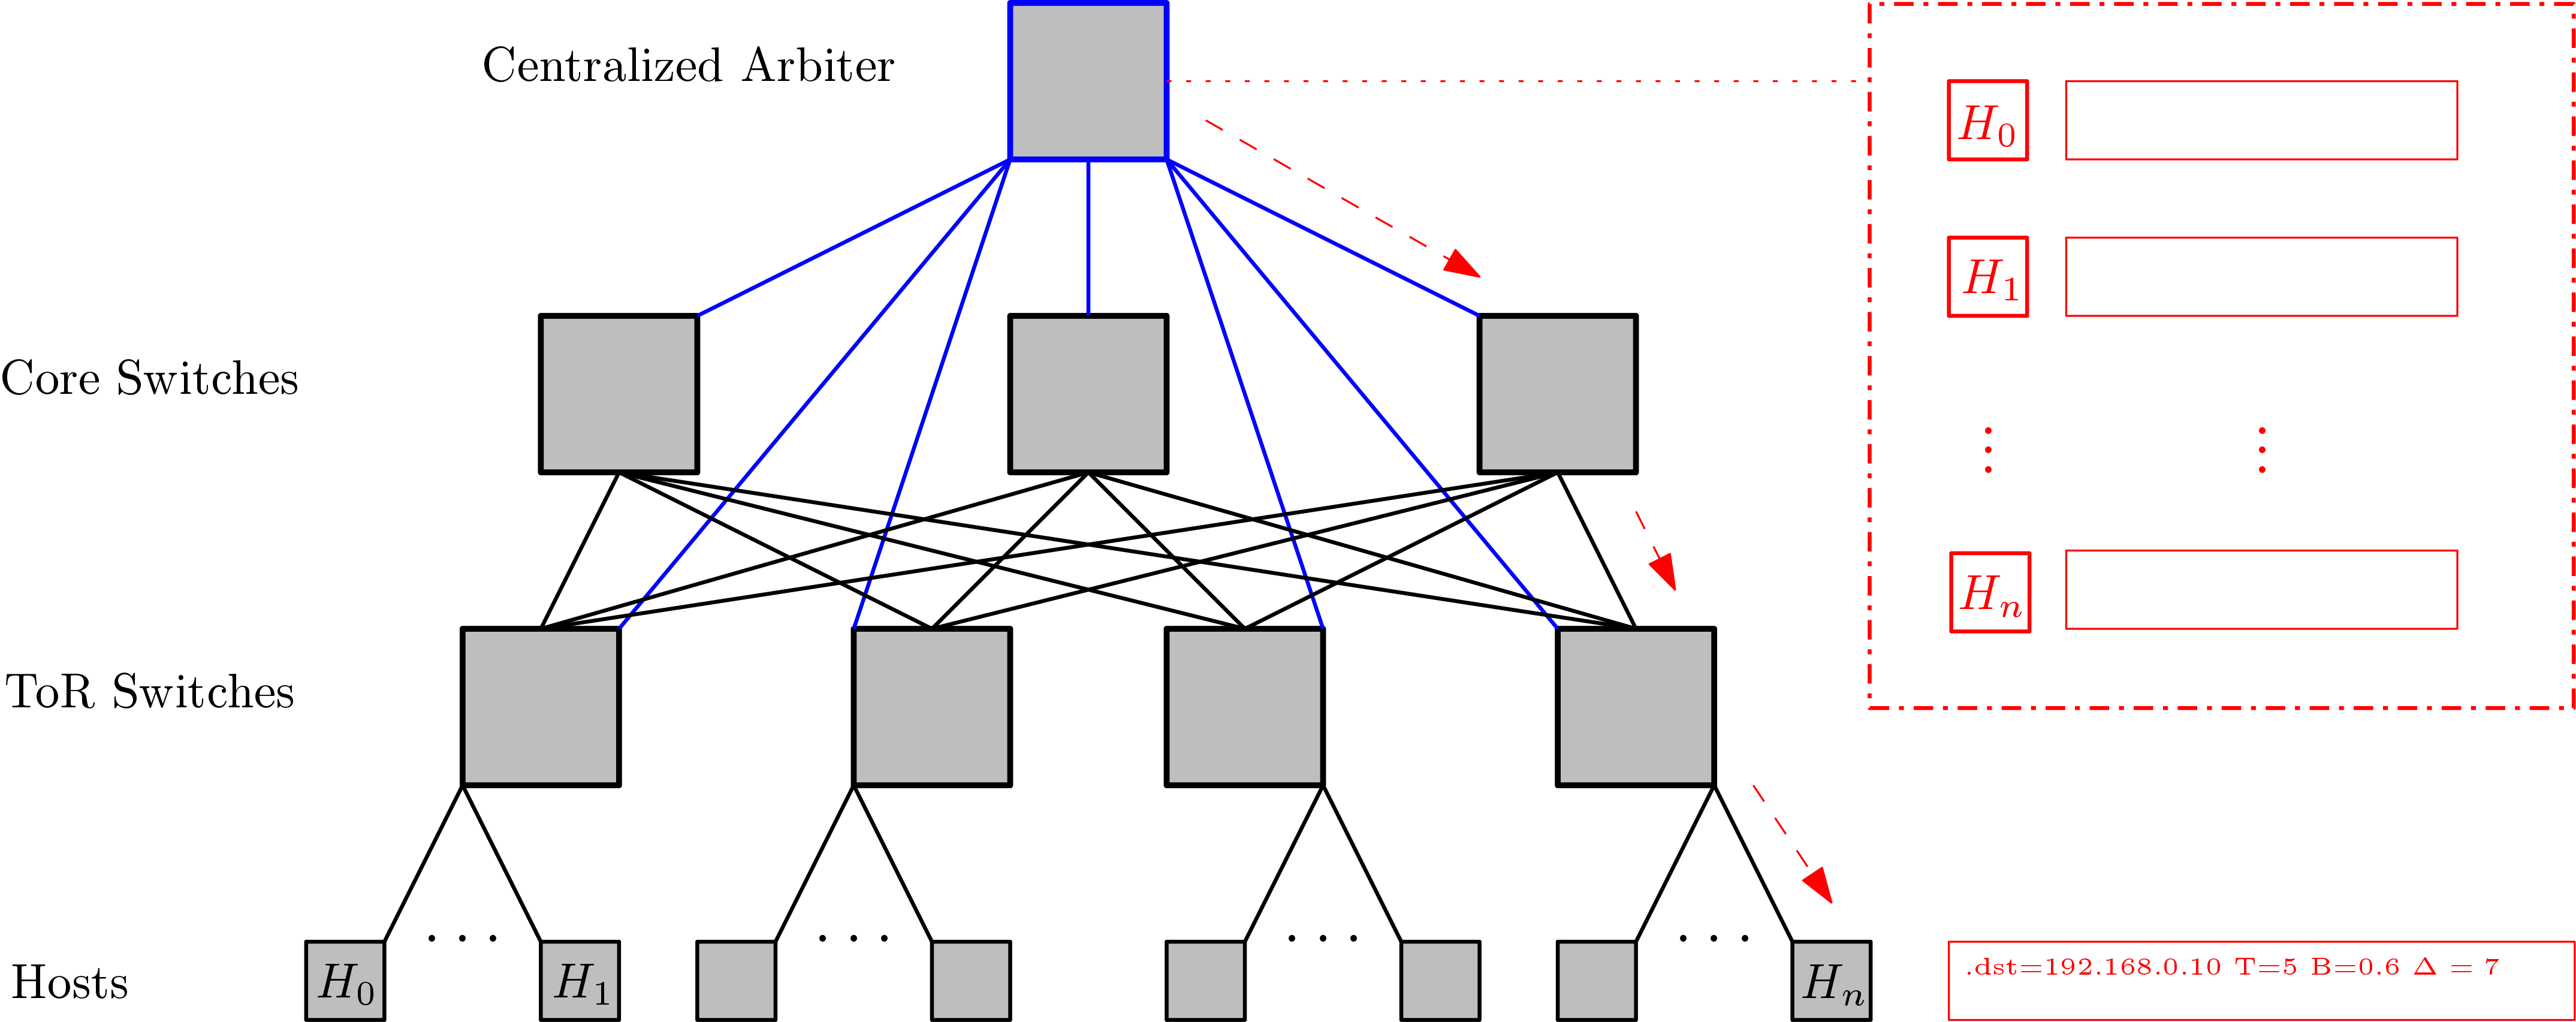
\includegraphics[width=1\linewidth]{Topology3}
\caption{Simple sketch of the Iroko architecture. A central scheduler maintains 
a consistent view of the current network activity and computes the optimal 
end-host bandwidth distribution. Bandwidth is enforced at end-hosts on a per-IP 
basis.}
\label{fig:Topology3}
\end{figure}

\subsection{Statistical System}
One potential implementation for our arbiter is to use reinforcement learning. 
In reinforcement learning, an agent (in our case the arbiter) performs actions 
in the environment and receives a reward signal from the environment to adjust 
its decisions in the next epoch ~\cite{Sutton:1998:IRL:551283}. The reward is 
generally used to represent the goal the agent is trying to achieve. The agent 
can freely choose whatever actions are necessary to achieve this goal 
~\cite{Sutton:1998:IRL:551283}.

The environment in this case is defined as the statistics collected from each 
switch. This decision is based on the fact that this data is easy to collect 
and provides a current snapshot of the performance of the network. We wish to 
optimize over the packet loss, and define the reward to be good if packet loss 
is decreasing (+1 reward); bad if it is increasing ( -1 reward); and acceptable 
if packet loss remains the same within a threshold (0 reward). Using this 
representation, we take full advantage of all the information provided in our 
data center; This representation is replicable and can be applied beyond the 
scope of this project.
 
Given the data center assumption, the number of end-hosts is known in the 
topology. We can define our arbiter's actions as a discretized representation 
among an n-dimensional vector where each cell is one of three values: increase 
decrease, or maintain the allocated bandwidth. This representation offers 
sufficient complexity. There are $3^n$ possible actions to perform and to 
achieve optimal results the agent must explore the environment extensively, 
precluding a significantly larger action space.

A potential improvement to our representation is a hierarchical learning agent. 
In this case, our arbiter would manage agents for each host and these 
sub-agents would manage their respective host whether to increase, decrease, or 
maintain bandwidth for their particular host. This problem can be referred to 
as hierarchical reinforcement learning~\cite{Borga1993}, but may prove to be 
beyond the scope of our current proposed solution, although has the added 
benefit of solving a set of sub-problems to address the global problem of 
packet loss and simplifies the representation spaces in the sub-problems.

Thus we frame our problem as one which can now be solved using techniques in 
reinforcement learning. A classic algorithm to consider is the use of 
SARSA~\cite{Sutton:1998:IRL:551283}, which is an online temporal difference 
algorithm used in classical reinforcement learning problems. One advantage of 
SARSA is its online nature~\cite{Sutton:1998:IRL:551283} which promotes more 
conservative decisions. Given full representation of our environment and 
actions, we can store information in an artificial neural network which is 
another popular choice in reinforcement learning literature. This model would 
store the reward signal information that is used to make future action choices, 
and is a theoretically proven function approximator which has made intractable 
environmental representations manageable~\cite{Sutton:1998:IRL:551283}.


%Using this model, we hope to achieve near 0% packet loss and provide a 
%%solution that gets somebody fired at google for not having tried it first.





%%%%%%%%%%%%%%%%%%%%%%%%%%%%%%%%%%%%%%%%%%%%%%%%%%%%%%
\section{Implementation}
\subsection{Overview}

We emulate our system in Mininet~\cite{mininet} to observe traffic 
patterns and to appropriately rate-limit end-hosts. Mininet has proven itself to be 
a viable tool to model new congestion control 
algorithms~\cite{mininet_learning}, and helped us prototype our concept 
efficiently. We built our custom SDN controller Iroko which interacts with 
traditional OpenFlow software switches as well as end-hosts. End-hosts run 
a custom real-world traffic generation script which adjusts based on 
information packets sent by the controller.


\subsection{Topology Simulation}
We chose to use  Mininet, a python data center emulation API, to prototype Iroko. Mininet's implementation leverages the Linux kernel to provide a lightweight virtualization of a data center in a single machine ~\cite{mininet}. This allowed us to create a prototype of Iroko we can test quickly using limited amounts of hardware. Other methods of testing Iroko would require more resources, or specialized code specific to the testbed which cannot be deployed in a real system ~\cite{mininet}. In contrast, Mininet has allowed us to develop Iroko such that we could deploy it in a real system without re-implementation independent of testbed specific code. 

In the Mininet environment, we created a fat-tree topology consisting of 20 switches and 16 hosts . The 20 switches are configured into 5 pods as described in ~\cite{fattree}. This design choice was to allow a direct comparison to Hedera  ~\cite{hedera}, a global arbiter which uses flow statistics to re-route elephant flows. In ~\cite{hedera}, Hedera was evaluated  using a fat-tree topology as we have described, and this allows us to directly compare Iroko against Hedera's performance . 

Mininet’s lightweight virtualization also allows the API to scale such as to support bigger topologies which otherwise couldn’t be prototyped easily ~\cite{mininet}. This feature will be useful for future research, because we can then test Iroko on other topologies beyond the fat-tree topology we looked at in this work. 

\subsection{Data Collection }
Since we knew prior to testing which port connected to each host, we collected different data from port connections to each end-host. This was accomplished using the awk scripting language and the Linux tc qdisc command to collect information.

Awk is a text parsing language available on most Linux distributions by default. Our awk script reads the /proc/net/dev file on each interface to collect the currently used  bandwidth on a link. We then used this to calculate free bandwidth which is the difference between theoretical maximum bisection bandwidth, and the reported bandwidth on a link.

In addition, we used the following Linux command:\\
\texttt{tc -s qdisc show dev <interface>}\\
where \texttt{<interface>} is the current host we are polling from. Using the 
obtained text, we then applied regex expressions to collect the packet loss, 
packet overlimits, and interface queues. Each of these data provide further 
information to hint at the current state of the data center. Our goal was to 
eliminate dropped packets, and used this to help Iroko make rate-limiting 
decisions. Overlimit packets provides information on when a link goes over it’s 
allocated bandwidth, and adds a potentially useful feature for our controller 
to learn from. Interface queues provide Iroko with information on the queue 
length of the host, which measures how many packets are buffered to be 
processed.  These additional statistics we hoped would provide our controller 
enough data to make meaningful inferences of the appropriate bandwidth 
allocation to each host. 

\subsection{Bandwidth Allocation}
Iroko rate limits traffic at the applications level, and thus uses UDP instead of TCP to communicate with hosts. Traffic is generated using a custom load generation application we wrote which reads a traffic matrix shared among all the hosts and sends network traffic accordingly. Iroko manages the current allocated bandwidth per host by sending a controller packet which updates their current allocated bandwidth.


\subsection{Reinforcement Learning Algorithm}

We chose to use the deep deterministic policy gradient policy algorithm (DDPG) almost entirely as described in ~\cite{DDPG} . DDPG is a form of actor-critic reinforcement learning algorithm ~\cite{Sutton:1998:IRL:551283} which uses neural networks to approximate $Q(s,a)$, and learns the policy by taking the actor network gradients relative to the critic $Q(s,a)$ approximations ~\cite{DDPG}.  Our agent learns using replay memory, which is a technique that helps deep reinforcement learning algorithms learn by making the data uncorrelated via random batch sampling ~\cite{DQLearning}. This decision might be unnecessary for a data center where authors have suggested that data center traffic is inherently unpredictable ~\cite{microte} and this suggests that we could assume data center data is inherently uncorrelated. We recognize these findings may also give an upper limit to the expected performance of Iroko. 

To find the optimal values, an agent must balance exploiting the current best actions with exploring an environment with a new action which may lead to bigger future rewards ~\cite{Sutton:1998:IRL:551283}. Instead of the exploration approach used in ~\cite{DDPG}, we use $\epsilon-greedy\ learning$, where an agent takes the best action with probability $\epsilon$ and a random action with probability $1 - \epsilon$ ~\cite{Sutton:1998:IRL:551283}. Our random action is then defined as follows:

\[
noise = 
\begin{cases}

uniform(0,1), &\text{P(x = increase) = .333},\\
uniform(-1,0), &\text{P(x = decrease) = .3333},\\
0, & \text{(x = unchanged) = .3333}
\end{cases}
\]

where uniform(a,b) refers to taking a random value in the range between [a, b]
This means we will take the best predicted value $(.5 * 1 + .5 * .33) =  ~.66.6\%$  and will increase $P(x= increase) * P(\epsilon) = 16. 667\%$ of the time or decrease $P(x= decrease) * P(\epsilon) = 16. 667\%$ of the time. It should be noted that the action value is still clamped between -0.9 and 0.9 regardless of the noise introduced. Alternative exploration policies could be used, but this one was chosen due it’s simplicity, and theoretical capability to explore the whole action space if allowed to run indefinitely.

We represent a state from the data center as an array combining a bit vector corresponding to the current host and it's allocated bandwidth, free bandwidth, packet loss, packet overlimits, and queue length:

\[ [0 0 0 ... 1 ... 0 0, bandwidth, free bandwidth, packet loss, overlimit, queue length ] \]
The advantage of this is that Iroko will learn a policy which considers all hosts together in unified representation instead of using separate agents for each network which wouldn't consider bandwidth allocation to each separate host.

The action Iroko takes at each step is the amount to increase or decrease the current hosts allocated bandwidth. Iroko will generate an adjustment value clamped between $-.9 - .9$. We chose this value range, because we wanted to avoid host starvation.  Iroko then modifies the allocated bandwidth similar to the approach used in ~\cite{remy} for congestion windows by using the action with allocated bandwidth as follows:

\[bandwidth_{t+1}   \leftarrow bandwidth_t +  a_t * bandwidth_t\]

where a is the chosen bandwidth adjustment, t is the previous epoch, and t+1 is the new allocation. This representation could be  modified in a number of ways, such as forcing a minimum expected bandwidth, or add the capacity to starve a host.





%%%%%%%%%%%%%%%%%%%%%%%%%%%%%%%%%%%%%%%%%%%%%%%%%%%%%%
\section{Evaluation}
\label{sec:evaluation}

In the absence of a commercial data center, the implementation of our network 
design is going to be done on top of mininet with simulated FatTree topologies 
of varying size. We stress test with iPerf and simulate data center traffic 
using tcpreplay and packet traces provided by~\cite{traffic} .

To evaluate the general effectiveness of our system, we plan to measure against 
existing centralized as well as decentralized solutions.
The centralized design will be based on Hedera~\cite{hedera}, a common and 
influential datacenter scheduler. The decentralized congestion control 
mechanism will be DCTCP~\cite{dctcp}, a state-of-the-art TCP congestion 
algorithm.

Since we are primarily concerned about reducing the latency and packet drops 
while keeping utilisation at maximum, the measurements to get a good insight 
into how well the design can perform are as follows:
\begin{enumerate}

\item Latency: We are aiming for a low latency network which means that 99th 
percentile latency in the network across all flows should as low as possible. 
Latency should be measured when all hosts are sending packets at the maximum 
limit and also with random traffic patterns. There should be low latency even 
during sudden bursts as the transmission rate is limited by a base value.

\item Packet drop rate: Ideally this metric will approach zero, as the 
objective of Iroko is to minimize packet loss.

\item Fairness: Fairness can be tested by introducing a new host to a 
completely saturated network and increasing the transmission rate to see if all 
the hosts gets fair share of the total bandwidth. We are assuming all flows 
should be at equal priority. Differential priority is out of scope.

\item Responsiveness: This metric depends on the predictive power and 
efficiency of Iroko. It may be interesting to analyze the response time of the 
central scheduler compared to decentralized DCTCP and TCP. In addition, it is 
valuable to identify at what data center and flow size the central computing 
node of the network may become a bottleneck.

\item Network utilization: We will measure the used bandwidth and the total 
load on the hosts. These metrics can be measured by varying the load from each 
host. Load to utilization ratio should be 1 until the saturation point and 
after that utilization should stay stable at the maximum bisection bandwidth.
It is also important to check that there is no starvation happening in any 
host. This can be measured by simulating random traffic patterns and plotting 
residual bandwidth and excess load. We expect overall utilization to be lower 
compared to Hedera and DCTCP. Although Iroko will maximize goodput, we do not 
measure it on grounds of simplicity.

\end{enumerate}

As baseline we will also compare to the default TCP congestion algorithm to 
estimate how our scheduler fares against the default case. As our initial 
simple design is very constrained in its ability to route and control traffic 
we expect to achieve less overall optimality against DCTCP and Hedera, but 
still gain a substantial advantage over common TCP.

%%%%%%%%%%%%%%%%%%%%%%%%%%%%%%%%%%%%%%%%%%%%%%%%%%%%%%
\section{Discussion}
\label{sec:discussion}

Rather predictably, Iroko struggles on random traffic patterns, however we
do not see this as particularly concerning. Firstly \textit{Iroko} still outperforms
both DCTCP and ECMP implementations. Further, as these traffic patterns
were designed by the authors of the Hedera paper \cite{hedera}, it remains
likely these patterns are somewhat amenable to the Hedera implementation.
Finally random traffic patterns seem unlikely to be prevalent in a
datacenter context. While the general predictability of datacenter
traffic remains an area of open research, our results show that
if there is sufficient predictability, we do get results better than
random, and for truly random data, Iroko does no worse generally than
incumbent solutions. 

Our machine learning approach shows promise, but machine learning remains
largely a black-box discipline. This nature makes it difficult for us
to determine precisely which parameters to use, and what drives
the improvements we've seen. Our current machine learning approach
is remarkably light-weight and does not require vast resources
in our test network. A heavier handed approach may yield better
results, however these may come at the cost of scalability. 

%%%%%%%%%%%%%%%%%%%%%%%%%%%%%%%%%%%%%%%%%%%%%%%%%%%%%%
\section{Future Work}
\label{sec:future}

Predicting datacenter traffic online with machine learning shows promise, and we believe that 
future widely deployed datacenter traffic control mechanisms will include
machine learning in their toolkit. However, machine learning alone may not
be sufficient to achieve the best possible results. Machine learning
based central traffic controllers can benefit from dynamic flow
scheduling as well as further traffic engineering. Thus expanding
the Iroko framework to include flow rather than interface based 
predictions, or a combination of both, would be an interesting 
avenue to pursue. Combined with a robust routing algorithm, we
believe such a solution could show superior performance when
compared to virtually all currently existing solutions.

For large, long-running workloads that require significant 
network resources at the termination such as MAP-REDUCE
workloads, hosts may have very predictable completion times
for these jobs. In such cases, hosts could report these 
estimated completion times to the central controller,
allowing the controller to account for them pre-emptively
rather than trying to infer them, which may take a couple
of epochs, and therefore reduce efficiency. Such a
system would be complementary to Iroko and
allow for finer grained control. By taking further
host level input, Iroko could reason about individual 
flows, and allocate not only bandwidth, but also 
specific paths.

Finally employing a token or credit based system similar
to that explored in \cite{expresspass} might yield excellent
results when coupled with our machine learning based predictive
central controller. This would allow hosts more ability to manage
their own bandwidth with inter-temporal substitution of flows,
while still enforcing centralized predictive control.


%%%%%%%%%%%%%%%%%%%%%%%%%%%%%%%%%%%%%%%%%%%%%%%%%%%%%%
\section{Conclusion}
\label{sec:conclusion}

Iroko represents a first attempt at using machine learning
to predict data center traffic. The endeavour relies crucially
on data center traffic having enough structure to in fact allow
some level of prediction. Yet even for largely random traffic
Iroko showed decent results, often besting baseline solutions.
Iroko is only the opening salvo, but the attempt has merit. 
More work must be done before claims of superiority to all
incumbent solutions can be made, but there are reasons to be
optimistic. 

Machine learning is perhaps the king of "black-box" solutions, 
and it's efficacy is undeniable if sometimes misleading. While
the standoff between so called "white-box" and "black-box" is 
likely to continue for the foreseeable future, Iroko shows
that "black-box" solutions do have a role to play. It may turn
out that neither comes to rule, but rather future SDN's will 
employ both techniques to build ever more efficient solutions.
It may well turn out that the future is grey.





\bibliographystyle{ACM-Reference-Format}
\bibliography{Iroko_Report} 

\end{document}
